\chapter{Getting started}
\section{Installing QDSP DSL}
The QDSP language is a external domain specific language, provided as an eclipse plugin. To install the plugin in an existing eclipse through the ``Intsall new software...'' under the Help menu, using the eclipse update site listed in the end of this section. Note that the plug in is written to Eclipse Platform Version: 4.3.0 and are not tested on other versions of eclipse.

\begin{table}[H]
	\centering
		\begin{tabular}{ll}
			\textbf{Eclipse update site:} & \url{https://raw.github.com/QDSP/installsite/master}
		\end{tabular}
\end{table}

\section{Creating a QDSP project}
When eclipse is downloaded, and the plugin for the QDSP DSL is installed, you are ready to create the project. Open eclipse and choose your workspace.

\begin{figure}[H]
	\centering
		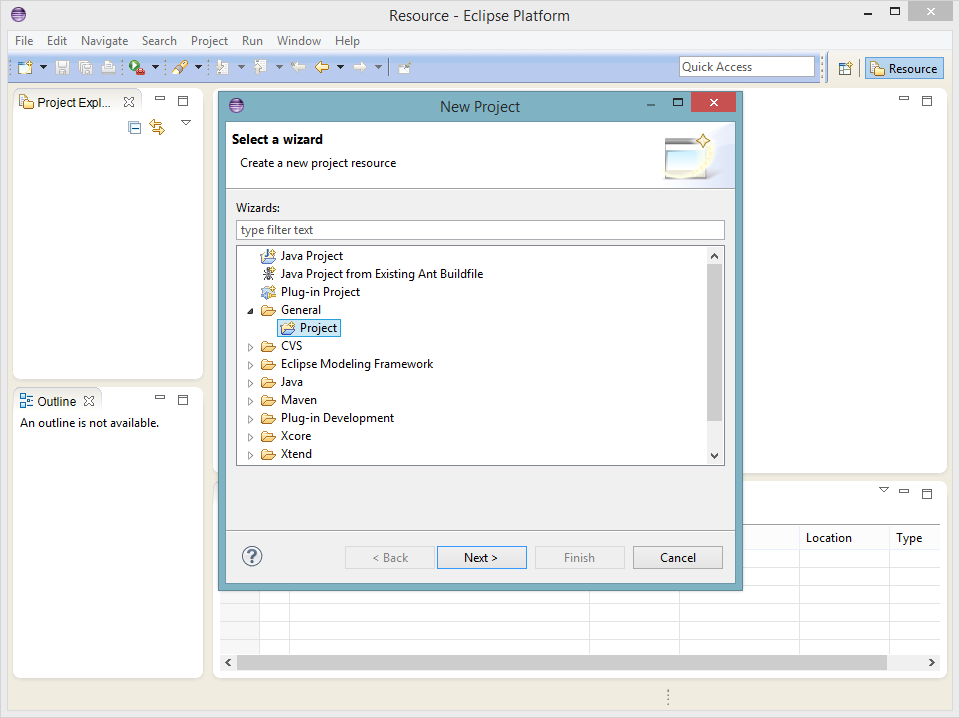
\includegraphics[width=0.8\textwidth]{newProject.png}
		\label{fig:newProject}
\end{figure}

\begin{itemize}[leftmargin=3cm]
	\item Go to File -> New and choose project
	\item Choose Project under General and click Next
	\item Enter a project title and click Finish
\end{itemize}

\begin{figure}[H]
	\centering
		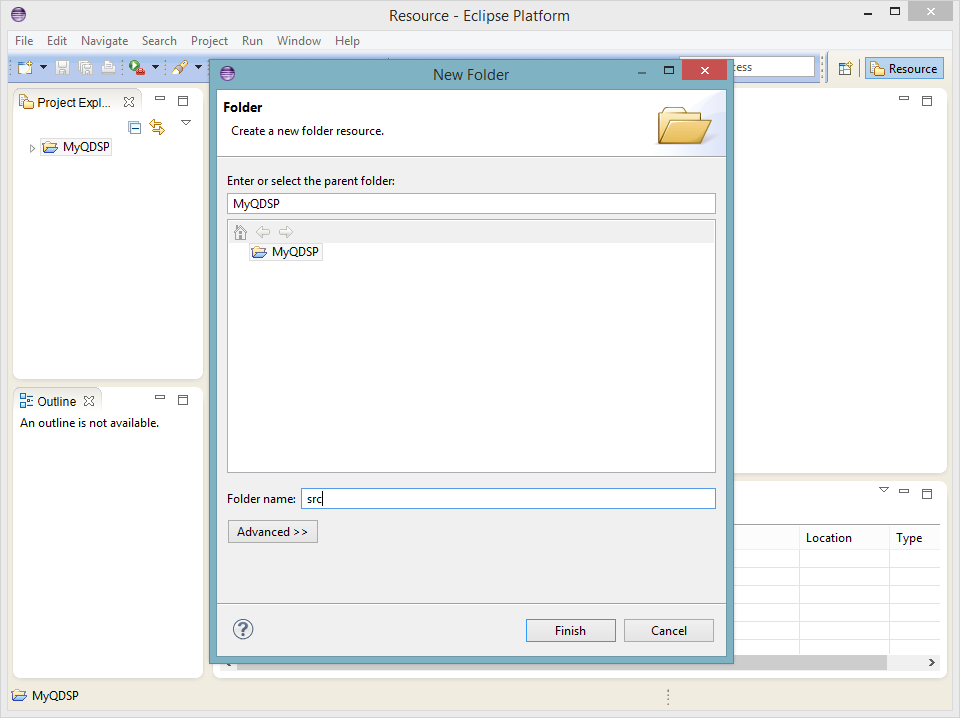
\includegraphics[width=0.8\textwidth]{newFolder.png}
		\label{fig:newFolder}
\end{figure}

\begin{itemize}[leftmargin=3cm]
	\item Rightclick project -> New and choose Folder
	\item Set folder name to ``scr'' and click Finish
\end{itemize}

\begin{figure}[H]
	\centering
		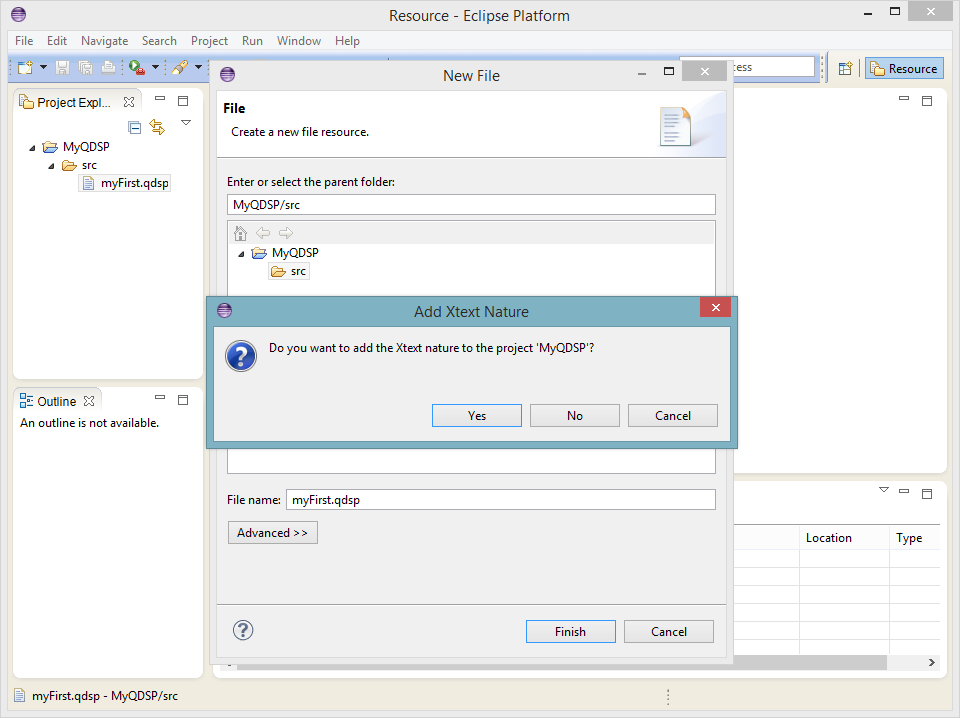
\includegraphics[width=0.8\textwidth]{newFile.png}
		\label{fig:newFile}
\end{figure}

\begin{itemize}[leftmargin=3cm]
	\item Rightclick scr -> New and choose File
	\item Enter file name and click Finish
	\item Click Yes in the ``Add Xtext Nature'' pop up
\end{itemize}

\section{Generated output}
The QDSP DSL compiler generates at least two files, a ``.qdspPro'' file containing the raw micro code for the written program, and a ``.vhdl'' file with a version of the QDSP3 optimized for the given micro code. This means that the size of heap  and the program memory is as small as possible, and the instruction set is trimmed to only contain the used instructions. The QDSP3 in the ``.vhdl'' file is already containing the microcode and the default values for the heap, and are therefor ready to use in a Xilinx ISE project. Just add the file to the project, and instantiate the module. All generated files can be found in the ``scr-gen'' folder.
 
\begin{figure}[H]
	\centering
		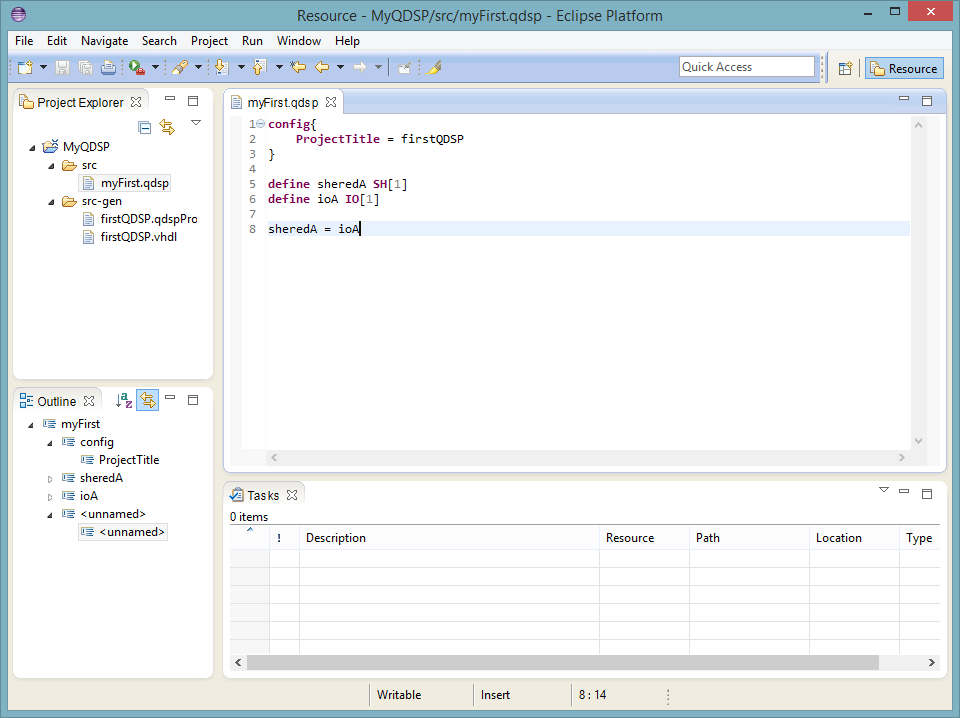
\includegraphics[width=0.8\textwidth]{out1.png}
		\label{fig:out1}
\end{figure}

If the run-time programming is enabled the size of heap  and the program memory is set to the values defined in the configuration. It also generates two more files. A ``.bin'' file containing a header telling the needed resources for the program to run, the micro code, and the default values for the heap. All of this is stored in a binary format. The last file ``qdspProgrammer.py'' is a Python script used to program the QDSP through Unity-Link or $\mu$TosNet. The programmer is specified to the configuration of the current QDSP.